\subsection{CRITERIA FOR CONVEXITY}

PROPOSITION 7. Let f be a finite real function defined on an interval \(I \subset R\) . For f to be convex on I it is necessary and sufficient that for every pair of numbers a, b of I such that a \textless{} b, and for every real number \(\mu\) , the function \(f(x) + \mu x\) attains its supremum on \([a, b]\) at one of the points a, b.

The condition is necessary; indeed, since \(\mu x\) is convex on \(\mathbf{R}\) , the function \(f(x) + \mu x\) is convex on I; one can therefore restrict oneself to the case \(\mu = 0\) . Then, for

\[
x = \lambda a + (1 - \lambda) b \quad (0 \leqslant \lambda \leqslant 1),
\]

one has

\[
f (x) \leqslant \lambda f (a) + (1 - \lambda) f (b) \leqslant \operatorname{Max} (f (a), f (b)).
\]

The condition is sufficient. Let us take \(\mu = -\frac{f(b) - f(a)}{b - a}\) and let \(g(x) = f(x) + \mu x\) ; one has \(g(a) = g(b)\) and therefore \(g(x) \leqslant g(a)\) for all \(x \in [a, b]\) , and one can check immediately that this inequality is equivalent to the inequality (1) where one replaces \(z\) by \(a\) and \(x'\) by \(b\) .

PROPOSITION 8. For a finite real function f to be convex (resp. strictly convex) on an open interval \(I \subset R\) it is necessary and sufficient that it be continuous on I, have a derivative at every point of the complement B relative to I of a countable subset of this interval, and that the derivative be increasing (resp. strictly increasing) on B.

The condition is necessary, from prop. 6 and its corollary 2 (I, p.~27); let us show that it is sufficient. Suppose, therefore, that \(f'\) is increasing on B, and that \(f\) is not convex; there then exist (I, p.~27, prop. 5) three points \(a, b, c\) of I, such that \(a < c < b\) , and \(\frac{f(c) - f(a)}{c - a} > \frac{f(b) - f(c)}{b - c}\) ; but from the mean value theorem (I, p.~14, th. 1) one has

\[
\frac {f (c) - f (a)}{c - a} \leqslant \sup _ {x \in \mathrm{B}, a <   x <   c} f ^ {\prime} (x) \quad \text { and } \quad \frac {f (b) - f (c)}{b - c} \geqslant \inf _ {x \in \mathrm{B}, c <   x <   b} f ^ {\prime} (x).
\]

One thus has \(\sup_{x\in \mathbf{B},a < x < c}f'(x) > \inf_{x\in \mathbf{B},c < x < b}f'(x)\) , contrary to the hypothesis that \(f'\) is increasing on B.

If now we assume that \(f'\) is strictly increasing on B, then \(f\) is convex and cannot be equal to an affine linear function on any open interval contained in I, for then \(f'\) would be constant on this interval, contrary to the hypothesis.

COROLLARY. Let \(f\) be a finite real function, continuous and twice differentiable on an interval \(\mathbf{I} \subset \mathbf{R}\) ; for \(f\) to be convex on \(\mathbf{I}\) it is necessary and sufficient that \(f''(x) \geqslant 0\) for all \(x \in \mathbf{I}\) ; for \(f\) to be strictly convex on \(\mathbf{I}\) it is necessary and sufficient that the previous condition be satisfied and further that the set of points \(x \in \mathbf{I}\) where \(f''(x) > 0\) be dense in \(\mathbf{I}\) .

This follows immediately from the preceding proposition, and from the corollary at I, p.~14.

Example. *On the interval {]}0, +∞{[} the function \(x^r\) (r any real number) has a second derivative equal to \(r(r - 1)x^{r - 2}\) ; thus it is strictly convex if \(r > 1\) or \(r < 0\) , and strictly concave if \(0 < r < 1\) .*

In order to be able to formulate another criterion for convexity we make the following definition: given the graph G of a finite real function defined on an interval \(I \subset R\) and an interior point a of I, we shall say that a line D passing through \(M_{a} = (a, f(a))\) is locally above (resp. locally below) G if there exists a neighbourhood \(V \subset I\) of a such that every point of D contained in \(V \times R\) is above (resp. below) G; we shall say that D is locally on G at the point \(M_{a}\) if there is a neighbourhood \(V \subset I\) of a such that the intersection of D and \(V \times R\) is identical to that of G and \(V \times R\) (in other words, if D is simultaneously locally above and locally below G).

PROPOSITION 9. Let f be a real finite function which is upper semi-continuous on an open interval \(I \subset R\) . For f to be convex on I it is necessary and sufficient that for every point \(M_{x}\) of the graph G of f every line locally above G at this point should be locally on G (at the point \(M_{x}\) ).

The condition is necessary: indeed, if \(f\) is convex on \(I\) then at every point \(\mathbf{M}_a\) of the graph \(G\) of \(f\) there exists a support line \(\Delta\) to \(G\) ; now \(\Delta\) is below \(G\) , so a fortiori locally below \(G\) (I, p.~29); if a line \(D\) is locally above \(G\) at the point \(\mathbf{M}_a\) it is locally above \(\Delta\) , so must coincide with \(\Delta\) , and consequently is locally on \(G\) at the point \(\mathbf{M}_a\) .

The condition is sufficient. Indeed, suppose it is satisfied, and suppose that \(f\) is not convex on I; then there are two points \(a, b\) of I ( \(a < b\) ) such that there are points \(\mathbf{M}_x\) of G strictly above the segment \(\mathbf{M}_a\mathbf{M}_b\) (fig.~4). In other words, the function \(g(x) = f(x) - f(a) - \frac{f(b) - f(a)}{b - a} (x - a)\) takes values \(>0\) on {[}a, b{]}; since \(g\) is finite and upper semi-continuous on this compact interval its least upper bound \(k\) on {[}a, b{]} is finite and \(>0\) , and

\pandocbounded{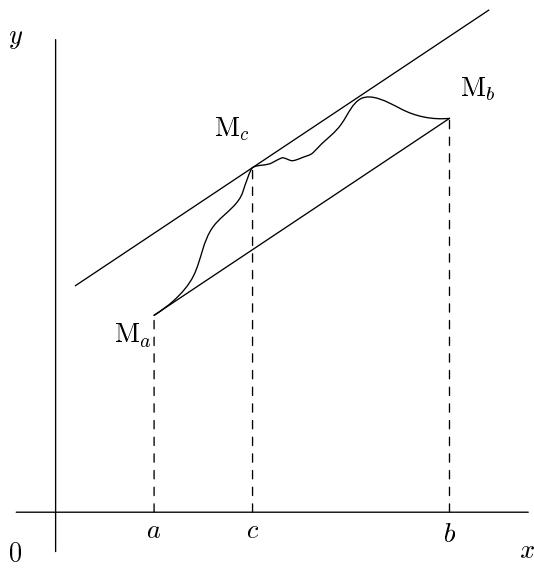
\includegraphics[keepaspectratio]{images/part001_3bcb0893.jpg}}\\
Fig. 4

the set \(\overline{g}(k)\) is closed and not empty (Gen.~Top., IV, p.~361, th. 3 and prop. 1). Let c be the greatest lower bound of \(\overline{g}(k)\) ; we have a \textless{} c \textless{} b, and at the point \(M_{c}\) the line D with equation \(y = f(c) + \frac{f(b) - f(a)}{b - a}(x - c)\) lies locally above G; but it cannot be locally on G at this point, since, for a \textless{} x \textless{} c, one has \(g(x) < k\) , which signifies that \(M_{x}\) is strictly below D. This has led us to a contradiction, which establishes the proposition.

COROLLARY 1. For a real finite function \(f\) defined on an open interval \(\mathbf{I} \subset \mathbf{R}\) and upper semi-continuous on \(\mathbf{I}\) to be convex on \(\mathbf{I}\) it is necessary and sufficient that for all \(x \in \mathbf{I}\) there should exist an \(\varepsilon > 0\) such that the relation \(|h| \leqslant \varepsilon\) entails

\[
f (x) \leqslant \frac {1}{2} (f (x + h) + f (x - h)).
\]

We have only to show that the condition is sufficient. Indeed, if at a point \(M_{a}\) of the graph G of f a line D is locally above G, then it is locally on G at this point; for, in the opposite case, for example, a point \(M_{a+h}\) would be strictly below D, while a point \(M_{a-h}\) would be below D; the mid-point of the segment \(M_{a-h}M_{a+h}\) would thus be strictly above D (fig.~5), and, in virtue of the hypothesis, \(M_{a}\) would a fortiori be strictly below D, which is absurd.

\pandocbounded{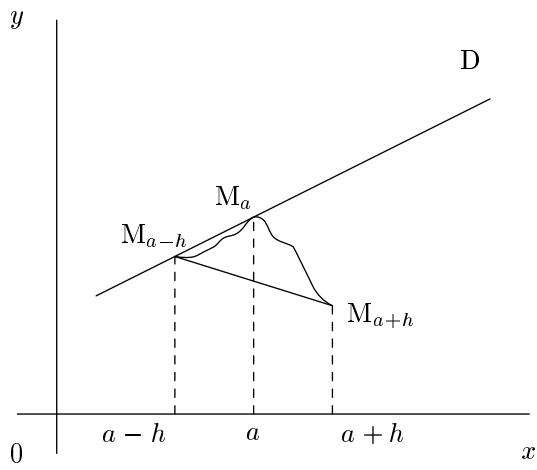
\includegraphics[keepaspectratio]{images/part001_b7dc5930.jpg}}\\
Fig. 5

COROLLARY 2. Let \(f\) be a finite real function defined on an open interval \(\mathrm{I} \subset \mathbf{R}\) . If for every point \(x \in \mathrm{I}\) there is an open interval \(\mathrm{J}_x \subset \mathrm{I}\) containing \(x\) and such that the restriction of \(f\) to \(\mathrm{J}_x\) is convex on \(\mathrm{J}_x\) , then \(f\) is convex on \(\mathrm{I}\) .

It is clear that \(f\) satisfies the criterion of prop. 9.

\setcounter{exercisegroup}{0}
\refstepcounter{exercisegroup}
